\documentclass[review, 12pt]{elsarticle}

\usepackage{lineno,hyperref}
\modulolinenumbers[1]

\journal{European Urology}
%\usepackage{fancyhdr}
%\rhead{\thepage}
\usepackage{fancyhdr}
\pagestyle{fancy}
\fancyhf{}
\renewcommand{\headrulewidth}{0pt}
\fancyhead[R]{\thepage}

%\usepackage{fig2vect}
\usepackage{graphicx}
%\usepackage{svg}
\usepackage{booktabs}
%\usepackage[swedish, english]{babel}

%%%%%%%%%%%%%%%%%%%%%%%
%% Elsevier bibliography styles
%%%%%%%%%%%%%%%%%%%%%%%
%% To change the style, put a % in front of the second line of the current style and
%% remove the % from the second line of the style you would like to use.
%%%%%%%%%%%%%%%%%%%%%%%

%% Numbered
%\bibliographystyle{model1-num-names}

%% Numbered without titles
%\bibliographystyle{model1a-num-names}

%% Harvard
%\bibliographystyle{model2-names.bst}\biboptions{authoryear}

%% Vancouver numbered
%\usepackage{numcompress}\bibliographystyle{model3-num-names}

%% Vancouver name/year
%\usepackage{numcompress}\bibliographystyle{model4-names}\biboptions{authoryear}

%% APA style
%\bibliographystyle{model5-names}\biboptions{authoryear}

%% AMA style
\usepackage{numcompress}\bibliographystyle{model6-num-names}

%% `Elsevier LaTeX' style
%\bibliographystyle{elsarticle-num}
%%%%%%%%%%%%%%%%%%%%%%%

\begin{document}

\begin{frontmatter}

\title{A Ready To Use Web-Application Providing a Personalized Biopsy Schedule for Men With Low-Risk PCa Under Active Surveillance\tnoteref{wordcount}}
\tnotetext[wordcount]{Word count abstract (headings excluded): 300; Word count text: 2484}

%% Group authors per affiliation:
\author[1]{Anirudh Tomer\corref{corauthor}, MSc} 
\cortext[corauthor]{Corresponding author (Anirudh Tomer): Erasmus MC, kamer flex Na-2823, PO Box 2040, 3000 CA Rotterdam, the Netherlands. Tel: +31 10 70 43393}
\ead{a.tomer@erasmusmc.nl}

\author[2]{Daan Nieboer, MSc}
\ead{d.nieboer@erasmusmc.nl}

\author[3]{Monique J. Roobol, PhD}
\ead{m.roobol@erasmusmc.nl}

\author[4]{Anders Bjartell, MD, PhD}
\ead{anders.bjartell@med.lu.se}

\author[2,5]{Ewout W. Steyerberg, PhD}
\ead{e.w.steyerberg@lumc.nl}

\author[1]{Dimitris Rizopoulos, PhD}
\ead{d.rizopoulos@erasmusmc.nl}

\author[6]{Movember Foundation’s Global Action Plan Prostate Cancer Active Surveillance (GAP3) consortium}

\address[1]{Department of Biostatistics, Erasmus University Medical Center, Rotterdam, the Netherlands}
\address[2]{Department of Public Health, Erasmus University Medical Center, Rotterdam, the Netherlands}
\address[3]{Department of Urology, Erasmus University Medical Center, Rotterdam, the Netherlands}
\address[4]{Department of Urology, Sk\r{a}ne University Hospital, Malm\"{o}, Sweden}
\address[5]{Department of Biomedical Data Sciences, Leiden University Medical Center, Leiden, the Netherlands}
\address[6]{The Movember Foundation’s Global Action Plan Prostate Cancer Active Surveillance (GAP3) consortium members presented in Appendix A}

%% or include affiliations in footnotes:

% !TEX root =  ../main_manuscript.tex 
\begin{abstract}
\texttt{Objective}: To develop a model and methodology for predicting the risk of Gleason \emph{upgrading} in prostate cancer active surveillance (AS) patients, and using the predicted risks to create risk-based \emph{personalized} biopsy schedules as an alternative to one-size-fits-all schedules (e.g., annually). Furthermore, to assist patients and doctors in making shared decisions of biopsy schedules, by providing them quantitative estimates of the \emph{burden} and \emph{benefit} of opting for personalized versus any other schedule in AS. Last, to externally validate our model and implement it along with personalized schedules in a ready to use web-application.\\

\texttt{Materials and Methods}: We used longitudinal prostate-specific antigen (PSA) measurements, timing and results of previous biopsies, and age at baseline from the world's largest AS study, Prostate Cancer Research International Active Surveillance or PRIAS (7813 patients, 1134 experienced upgrading). We fitted a Bayesian joint model for time-to-event and longitudinal data to the PRIAS dataset. We then externally validated our model in the largest six AS cohorts of the Movember Foundation's Global Action Plan (GAP3) database (${>20,000}$ patients, 27 centers worldwide), covering nearly 73\% of all GAP3 patients. We used the predicted upgrading-risks from the validated models to schedule biopsies whenever a patient's risk of upgrading was above a certain threshold. To assist patients in choice of this threshold to compare the resulting schedule with currently practiced schedules, we provided them the timing and the total number of biopsies (burden) planned, and the predicted time delay in detecting upgrading (shorter is better) for each schedule.\\

\texttt{Results}: The cause-specific cumulative upgrading-risk at year five of follow-up was 35\% in PRIAS, and at most 50\% in GAP3 cohorts. In the PRIAS based model, PSA velocity was a stronger predictor of upgrading (Hazard~Ratio:~2.47, 95\%CI:~1.93--2.99) than PSA value (Hazard~Ratio:~0.99, 95\%CI:~0.89--1.11). Our model had a moderate area under the receiver operating characteristic curve (0.6--0.7) in validation cohorts. The prediction error was moderate (0.1--0.2) in GAP3 cohorts where the impact of PSA value and velocity on upgrading-risk was similar to PRIAS, but large (0.2--0.3) otherwise. Our model required recalibration of baseline upgrading-risk in validation cohorts. We used predicted upgrading-risk from the validated model to create personalized biopsy schedules for real AS patients and implemented them in a web-application (\url{http://tiny.cc/biopsy}).\\

\texttt{Conclusions}: We successfully developed and validated a model for predicting upgrading-risk, and providing risk-based personalized biopsy decisions, in prostate cancer AS. Personalized prostate biopsies are a novel alternative to fixed one-size-fits-all schedules that may help to reduce unnecessary prostate biopsies while maintaining cancer control. The model and schedules made available via a web-application enable shared decision making of biopsy schedules by comparing fixed and personalized schedules on total biopsies and expected time delay in detecting upgrading.
\end{abstract}
%Word count: 299 words excluding headings

\begin{keyword}
Active Surveillance\sep Biopsies \sep Personalized Medicine\sep Prostate Cancer \sep Shared Decision Making
\end{keyword}

\end{frontmatter}

\linenumbers

% !TEX root =  ../main_manuscript.tex 
\section{Introduction}
\label{sec:introduction}
Chronic non-communicable diseases (e.g., cancer, renal, cardiovascular diseases, etc.) are the primary cause of human deaths worldwide~\citep{alwan2010monitoring}. After diagnosis, in many such patients, surveillance tests are performed periodically to detect disease \textit{progression}, a non-terminal event. Often the most accurate or gold standard surveillance tests are also invasive. For example, to diagnose progression, biopsies are conducted repeatedly in prostate cancer~\citep{bokhorst2015compliance}, endoscopies in Barrett's esophagus~\citep{streitz1993endoscopic}, and colonoscopies in colorectal cancer~\citep{krist2007timing}. Repeat biopsies are also utilized to detect allograft deterioration in lung~\citep{mcwilliams2008surveillance} and kidney transplant~\citep{henderson2011surveillance} patients.

Usually, invasive tests are scheduled in a fixed manner, e.g., every six months. Test frequency varies between diseases~\citep{henderson2011surveillance,bokhorst2015compliance,krist2007timing} and cohorts. Although, due to the periodical nature of test schedules, progression is always detected with a time delay (Figure~\ref{fig:delay_explanation}). This time delay can be reduced by scheduling tests frequently. However, invasive tests are difficult to conduct, can lead to severe complications~\citep{loeb2013systematic,krist2007timing}, cause patient discomfort, and sometimes patients may not comply with frequent tests~\citep{bokhorst2015compliance}. In this regard, fixed test schedules ignore the differences in speed of progression between patients, and impose an equal medical burden on all. Hence, the frequency of invasive tests holds important implications for patients.

\begin{figure}
\centerline{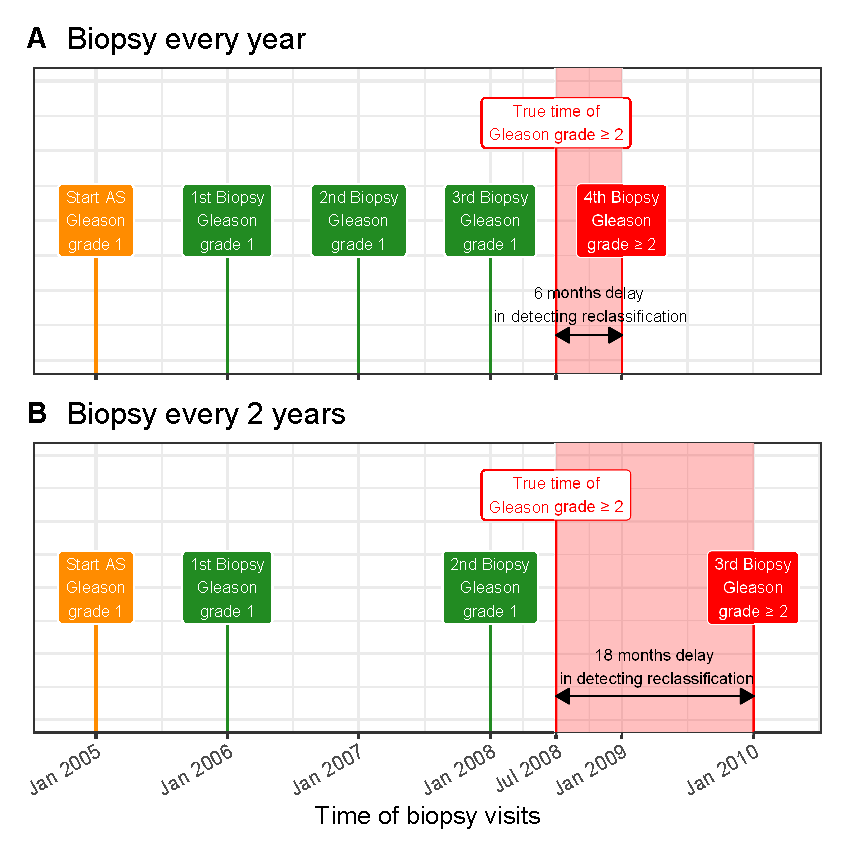
\includegraphics{images/delay_explanation.eps}}
\caption{\textbf{Trade-off between the number of invasive tests and time delay in detecting progression (non-terminal event of interest):} The true time of progression for this patient July 2004. More frequent invasive tests in \textbf{Panel~A} lead to a smaller time delay in detection of progression than less frequent invasive tests in \textbf{Panel~B}. Since invasive tests are conducted periodically, the time of progression is observed as an interval. For example, between Jan~2004--Jan~2005 in \textbf{Panel~A} and between Jan~2004--Jan~2006 in \textbf{Panel~B}.} 
\label{fig:delay_explanation}
\end{figure}

In this paper, we aim to balance the number of invasive tests (burden) and the time delay in detection of \textit{progression} (less is beneficial) better than fixed schedules. For this purpose, we intend to create personalized test schedules that exploit patient-specific clinical data accumulated during follow-up. This data includes baseline characteristics of patients; results from previous invasive tests; and longitudinal biomarker, physical examination, and medical imaging measurements, etc. Previous approaches for personalized schedules may be divided into three categories. First, heuristic methods such as decision making flowcharts, e.g.,~\citet{bokhorst2015compliance}. However, flowcharts discretize continuous clinical outcomes, often utilize only the latest data point, and ignore the measurement error in observed outcomes. Second, personalized test decisions employing partially observable Markov decision processes~\citep{alagoz2010operations, steimle2017markov}. Although, their application with continuous outcomes is limited by the curse of dimensionality. Third, personalized schedules obtained by optimizing a loss function of clinical parameters of interest~\citep{bebu2017optimal,rizopoulos2015personalized}, including our previous work on scheduling biopsies in prostate cancer~\citep{tomer2019personalized}. In this work, we will employ the third approach.

First, we develop a full specification of the joint distribution of patient-specific longitudinal clinical outcomes and time of \textit{progression}. We achieve this using joint models for time-to-event and longitudinal data~\citep{tsiatis2004joint,rizopoulos2012joint}. We use joint models because they are inherently personalized. Specifically, they exploit patient-specific random effects~\citep{laird1982random} to model longitudinal outcomes without discretizing them. We subsequently employ the fitted joint model for new patients, to estimate their patient-specific cumulative-risk over their current and future follow-up visits. These risk predictions utilize their clinical data accumulated until their latest follow-up. We then schedule invasive tests on all those future follow-up visits where a patient's conditional cumulative-risk of progression is above a certain threshold (e.g., 10\% risk). We also automate the choice of this threshold and the resulting schedule. More specifically, we optimize a function of the number of tests in a schedule and the expected time delay in the detection of progression. We estimate this delay in a patient-specific manner for both fixed and personalized schedules, thus facilitating shared-decision making of invasive test schedules.

This research is motivated by the problem of scheduling biopsies~\citep{nieboer2018active} in the world's largest prostate cancer active surveillance study PRIAS~\citep{bokhorst2015compliance}. It has 7813 patients, 104904 longitudinal measurements, and 1134 patients with cancer progression. Patients in PRIAS have low and very-low grade prostate cancer, often over-diagnosed due to prostate-specific antigen (PSA) based screening tests~\citep{crawford2003epidemiology}. The goal of surveillance is to delay serious treatments (e.g., surgery, chemotherapy, etc.) until cancer progression is observed. For this purpose, patients are monitored continually via PSA (ng/mL) blood tests, digital rectal examination (DRE) for shape and size of the tumor, and biopsy Gleason grade group~\citep{epsteinGG2014}. The latter is the strongest indicator of cancer-related outcomes. Consequently, treatment is commonly advised upon observing an increase in a patient's biopsy Gleason grade group (cancer progression). Currently, the most common biopsy schedule of yearly biopsies~\citep{loeb2014heterogeneity} leads to many unnecessary biopsies in slow/non-progressing patients (50\% proportion in some cohorts). Biopsy burden combined with patient non-compliance to frequent biopsies~\citep{bokhorst2015compliance} has raised concerns regarding the optimal biopsy schedule. Since prostate cancer has the second highest incidence among all cancers in males~\citep{GlobalCancerStats2012}, biopsy schedules tailored for individual patients can reduce the overall burden of biopsies in a large number of patients worldwide.

The rest of the paper is as follows. Section~\ref{sec:jointmodel} briefly introduces the joint modeling framework. In Section~\ref{sec:schedule} we present the methodology for personalized schedules, and then demonstrate them for biopsies in real PRIAS patients in Section~\ref{sec:results}. Lastly, in Section~\ref{sec:sim_study} we show the efficacy of personalized schedules via a realistic simulation study based on PRIAS patients.
%Intro: 517 words
%Cumsum: 517 words
% !TEX root =  ../main_manuscript.tex 
\section{Patients and Methods}

\subsection{Study Cohort}
Prostate Cancer International Active Surveillance (PRIAS) is an ongoing prospective cohort study of men with low- and very-low risk PCa diagnoses \cite{bul2013active}. More than 100 medical centers from 17 countries contribute in PRIAS, using a common study protocol (\url{www.prias-project.org}). We used the data collected between December~2006 (beginning of PRIAS study) and May~2019. The PSA was measured every three months until year two of follow-up and every six months thereafter. Biopsy schedule was year one, four, seven, and ten, and additional yearly biopsies when PSA doubling time was between zero and ten years. The primary event used in this work is Gleason~$\geq$~7 (GS7) because it is commonly used as a trigger for treatment advice. It was observed in 1134 patients. However, 2250 patients were provided treatment (see Table \ref{table:prias_summary}). Treatment in absence of GS7 may have been advised on the basis of PSA, number of biopsy cores with cancer, anxiety, or other reasons. We focused only on GS7 because of its strong association with cancer-related outcomes. Due to the periodical nature of biopsies, the time of GS7 was only available as a time interval in which GS7 occurred.

\begin{table}
\small\sf\centering
\caption{\textbf{Patient characteristics for the PRIAS dataset}. The primary event of interest is Gleason~$\geq$~7. IQR: interquartile range, PSA: prostate-specific antigen.}
\label{table:prias_summary}
\begin{tabular}{lr}
\hline
\hline
Characteristic & Value\\
\hline
Total patients & 7813\\
Gleason~$\geq$~7 (primary event) & 1134\\
Treatment & 2250\\
Watchful waiting & 334\\
Loss to follow-up & 250\\
Death (unrelated to prostate cancer) & 95\\
Death (related to prostate cancer) & 2\\
\hline
Median age at diagnosis (years) & 66 (IQR: 61--71)\\
Median follow-up period per patient (years) &  1.8 (IQR: 0.9--4.0)\\
Total PSA measurements & 67578\\
Median number of PSA measurements per patient &  6 (IQR: 4--12)\\
Median PSA value (ng/mL) & 5.7 (IQR: 4.1--7.7)\\
Total biopsies & 15686\\
Median number of biopsies per patient &  2 (IQR: 1--2)\\
\hline
\end{tabular}
\end{table}
%Study cohort: 225 words
%Cumsum: 742 words
% !TEX root =  ../main_manuscript.tex 
\subsection{Statistical Methods}
The goal of the statistical analysis of the PRIAS data was to develop a model for predicting the time of disease reclassification in a personalized manner. To this end, for each patient we have the information about his age at the start of AS, all observed PSA measurements, and the time of the last negative biopsy. 

We start by specifying a model which extracts the underlying $\log_2\{\mbox{PSA + 1}\}$ profile of each patient from the observed PSA measurements. More specifically, we specify a linear mixed effects model with $\log_2\{\mbox{PSA + 1}\}$ as the outcome (see Outcome--2 in Figure \ref{fig:jm_blockdiag}). Our model uses a separate non-linear $\log_2\{\mbox{PSA + 1}\}$ profile over time, for each patient. It employs patient-specific random effects to account for correlation between $\log_2\{\mbox{PSA + 1}\}$ measurements of the same patient. However, the PSA measurements of a patient may be higher when measured closer to the time of reclassification. This is especially an issue because PSA measurements are missing (non-random) once a patient obtains disease reclassification. The vice versa, that is, disease reclassification may be predicted by looking at the PSA is also valid. To model this two-way effect, we specify a model for time of reclassification which shares the random effects used in the model for PSA (see Figure \ref{fig:jm_blockdiag}). Particularly, we use a relative risk model, wherein the hazard of reclassification utilizes the shared random effects indirectly, by depending on the fitted $\log_2\{\mbox{PSA + 1}\}$ value and velocity (rate of change). This connected specification of a linear mixed model and relative risk model is commonly known as a joint model for time-to-event and longitudinal data \citep{rizopoulos2012joint,tomer2019,coley2017prediction}.

\begin{figure}[!htb]
\centerline{\includegraphics[width=\columnwidth]{images/jm_blockdiag.pdf}}
\caption{\textbf{Diagram of the joint model}: Per patient we observe the $\log_2\{\mbox{PSA + 1}\}$ transformed PSA, and the results of biopsies. We combine information from these observations to estimate the time of disease reclassification. To this end, we use a linear mixed effects model for $\log_2\{\mbox{PSA + 1}\}$ measurements, and proportional hazards model for time of disease reclassification. The time of disease reclassification depends on patient age, time of latest negative biopsy and underlying trend of PSA. To account for the correlation between PSA measurements and time of reclassification, the two models share patient-specific random effects in their model equations.}
\label{fig:jm_blockdiag}
\end{figure}

The consequence of such a joint model is that the shared random effects represent the unobservable state of PCa of each patient. On the other hand outcomes such as disease reclassification and PSA measurements are its observable manifestations. Such a shared random effect structure allows easy addition of more disease progression indicators (e.g., MRI information) when they are available in future. Furthermore, this structure also allows the follow-up schedule for outcomes/biopsies to depend on the observed values of each other. This is especially important because yearly biopsies in the PRIAS program are scheduled on the basis of the observed PSA doubling time of a patient.

We fit the joint model using the R package \textbf{JMbayes} \citep{rizopoulosJMbayes}. The package uses the Bayesian methodology to estimate model parameters. The model parameters and 95\% credible intervals are presented in Table.. of Appendix.

\subsection{Assessment of Predictions}
We assessed the goodness of fit of our model using both in-sample and out-of-sample predictions. For out-of-sample predictions we utilized the XX largest AS cohorts that constitute the GAP3 database \citep{gap3_2018}. That is, we used our model to predict disease reclassification in patients of other cohorts. The accuracy of these predictions were measured via the prediction error and the area under the receiver operating characteristic curves (AUC). The prediction error represents the difference between the true disease reclassification status of a patient, and the predicted risk of reclassification. Ideally this difference should be zero. On the other hand the AUC defines if the model is able to discriminate between patients who obtain reclassification versus those do not obtain reclassification. Ideally it should be equal to one. Since we work under a longitudinal study framework we compute these measures at a gap of every one year during the entire follow-up period.

\subsection{Decision Making Framework}
To assist patients and doctors in decision making for biopsies, we use the predicted risks of reclassification from our model. We calculate the probability if the patient will progress over the next ten years. We also provide an estimate of the number and time of biopsies that may be conducted, and the corresponding estimate of delay in detection of time of reclassification. Simultaneously, the patient is provided estimate of the number of time of biopsies with fixed schedule of biopsies. This allows patients to weigh harms and benefits of each strategy. We also implement this in a web-based risk calculator.
%Stat analysis: 336 words
%Cumsum: 1078 words
% !TEX root =  ../main_manuscript.tex 
\section{Results}
For patients in the PRIAS dataset, probability of obtaining reclassification within the first five and ten years is 33\% and 42\%, respectively (see Figure \ref{fig:npmle_plot}). That more than 50\% of the patients may not require any biopsy in the first ten years. We refer to them as \textit{slow progressing} patients hereafter. For every ten years increase in a patient age the corresponding adjusted hazard ratio of reclassification is 1.45~(95\%CI:~1.29--1.61). For an increase in fitted $\log_2\{\mbox{PSA + 1}\}$ value from the first quartile of fitted value (2.67) to the third quartile (2.82), the corresponding adjusted hazard ratio of reclassification is 1.00~(95\%CI:~0.98--1.02). On the other hand an increase in fitted $\log_2\{\mbox{PSA + 1}\}$ velocity from the first quartile of fitted velocity (-0.04) to the third quartile (0.15), the corresponding adjusted hazard ratio of reclassification is 2.45~(95\%CI:~1.83--2.95). These results indicate that the velocity of $\log_2\{\mbox{PSA + 1}\}$ measurements is a stronger predictor of hazard of reclassification than the $\log_2\{\mbox{PSA + 1}\}$ value.

The area under the receiver operating characteristic curves and the prediction error over time are shown.


%Stat analysis: 632 words
%Cumsum: 1710 words
% !TEX root =  ../main_manuscript.tex 
\section{Discussion}
We developed a novel methodology for personalized biopsies in low-risk PCa patients enrolled in AS programs. These biopsies are based on a patient's risk profile for having a Gleason $\geq$ 7 (GS7). To assist patients in making a choice between the personalized and currently practiced fixed schedules, we give objective estimates of the consequences of following each schedule. More specifically, for a schedule we give the total number of biopsies (burden), the time at which they will be conducted, and the expected delay in detection of GS7. This delay is estimated after accounting for the probability of not having any GS7 at all over the follow-up period. Lastly, our approach dynamically updates the aforementioned schedules and consequences as more patient data becomes available over follow-up.

The aforementioned methodology is based on the world's largest PCa AS program, PRIAS. Consequently, a lot of patients may get benefited from this study. To this end, we have developed a web-application implementing our methodology. The web-application only requires patient data in well known file formats (e.g., SPSS, CSV etc.), but does not require any separate integration with the electronic health record of the PRIAS program. We hope that this will lead to improvement in the shared decision making of biopsies, with patients having objective estimates of the consequences of their decisions. 

\textbf{Clinical implications:} The median survival time for GS7 is more than ten years in PRIAS. That is, more than 50\% patients do not require any biopsy during the first ten years of follow-up. The situation is similar in many other cohorts. Hence frequent biopsies may not be recommended for all patients.

Existing work on reducing the burden of biopsies in AS primarily advocates less frequent heuristic schedules of biopsies \citep{inoue2018comparative} (e.g., biopsies biennially instead of annually). To our knowledge, risk-based biopsy schedules have barely been explored yet in AS \citep{nieboer2018active,bruinsma2016active}. The part of our results pertaining to the fixed/heuristic schedules is comparable with corresponding results obtained in existing work \citep{inoue2018comparative}, even though the AS cohorts are not the same. Thus, we anticipate similar validity for the results pertaining to the personalized schedules.

Our work has certain limitations. The prediction model that we developed is valid only for the first thirteen years of follow-up in AS, whereas PCa in AS patients progresses slowly. This issue can be mitigated by refitting the model as more follow-up data is gathered in PRIAS. The results of external validation indicate that the use of our model may be restricted in cohorts with AUC, and RMSPE results similar to that of PRIAS. To this end, in other cohorts, refitting the model to their dataset will be required before making risk based schedules, and estimating the consequences of each schedule. There is also a potential for including diagnostic information from novel biomarkers, quality of life measures, and magnetic resonance imaging. Currently, this data is very sparsely available in the PRIAS dataset. However, in future, adding this information in our model is trivial. This is because modeling correlation for extra outcomes  (see Figure \ref{fig:jm_blockdiag}), mainly entails sharing the random effects in the joint model structure. Since MRI scans are expensive in developing countries, our model can also be used to trigger MRI scans. Lastly, in this study focus only on biopsy Gleason upgrade (reclassification). In this regard, accounting for competing risks (see Table \ref{table:prias_summary}), and for inter-observer variation \citep{coley2017prediction} in biopsy Gleason scores can be interesting to investigate further.
%Stat analysis: 679 words
%Cumsum: 2389 words
% !TEX root =  ../main_manuscript.tex 
\section{Conclusions}
We developed a novel methodology and statistical model for personalized scheduling of biopsies in prostate cancer active surveillance (AS) patients. Unlike fixed biopsy schedules, personalized schedules utilize a patient's risk of reclassification to decide biopsies. They also update as more patient data becomes available over follow-up. Our model is externally validated in largest five AS cohorts of the GAP3 database. Our methodology is implemented in a web-application (\url{https://emcbiostatistics.shinyapps.io/prias_biopsy_recommender/}) and is accessible to large number of AS patients from the validated cohorts. To assist patients/doctors in making a shared decision of an appropriate biopsy schedule, the web-application provides expected time delay in detection of reclassification (smaller is beneficial), and timing and total number of biopsies (burden), for both personalized and currently used fixed schedules.
%Conclusion: 95 words
%Cumsum: 2484 words

\input{mainmatter/author_contrib}
\section*{Acknowledgments}
The first and last authors would like to acknowledge support by Nederlandse Organisatie voor Wetenschappelijk Onderzoek (the national research council of the Netherlands) VIDI grant nr. 016.146.301, and Erasmus University Medical Center funding. Part of this work was carried out on the Dutch national e-infrastructure with the support of SURF Cooperative. The authors also thank the Erasmus University Medical Center's Cancer Computational Biology Center for giving access to their IT-infrastructure and software that was used for the computations and data analysis in this study.

This work was supported by the Movember Foundation. The funder did not play any role in the study design, collection, analysis or interpretation of data, or in the drafting of this paper.
\section*{Appendix A. Members of The Movember Foundation’s Global Action Plan Prostate Cancer Active Surveillance (GAP3) consortium}
\input{mainmatter/gap3members}

\bibliography{bibliography}

\end{document}